\documentclass{article}
\usepackage[utf8]{inputenc}
\usepackage{graphicx}
\usepackage{hyperref}
\hypersetup{colorlinks=true,
		urlcolor=blue}
\begin{document}

    \title{Abstract Classes and Interfaces: Practical Examples}
    \author{Andrew Lalis | \emph{a.lalis@student.rug.nl} \\
            George Argyrousis | \emph{g.argyrousis@rug.nl} }
    \date{Last modified: \today}

    \maketitle

    \section{Abstract Classes}
        \subsection{Definition}
        	\href{https://docs.oracle.com/javase/tutorial/java/IandI/abstract.html}{Oracle Abstract Classes and Methods Tutorial}

            An abstract class, in the context of Java, is a superclass that cannot be instantiated and is used to state or define general characteristics. An object cannot be formed from a Java abstract class; trying to instantiate an abstract class only produces a compiler error. The abstract class is declared using the keyword abstract.

            Subclasses extended from an abstract class have all the abstract class's attributes, in addition to attributes specific to each subclass. The abstract class states the class characteristics and methods for implementation, thus defining a whole interface.

        \subsection{Example}
            We will illustrate the abstract class functionality by creating a small application that should act as a model, creating a Student database for a University. We will begin by defining an \textbf{abstract} Human class that reflects the idea of the Human characteristics that would be universal in the database.

            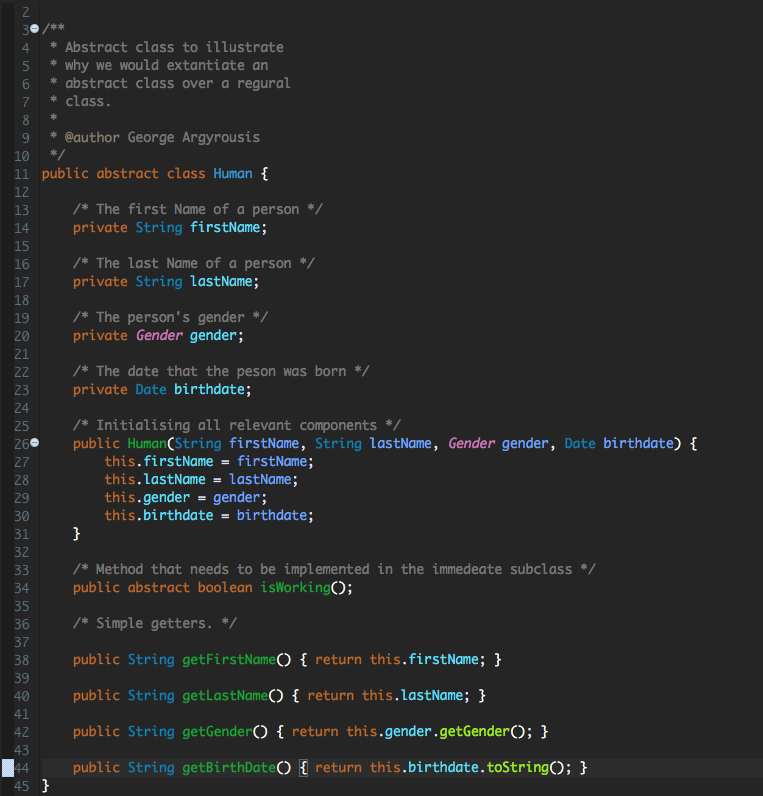
\includegraphics[scale=0.48]{images/Human.png}

            We have defined attributes such as \textit{firstName}, \textit{lastName}, \textit{gender} and \textit{birthdate}. Representing common attributes among all humans. We have also defined one abstract method that will be implemented when the abstract class is extended by another regular class.

            Of course we would not be able to create a \textbf{Human} object.

            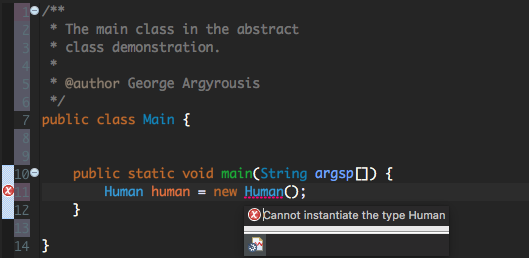
\includegraphics[scale=0.7]{images/Main_error.png}

            Human is an abstract class that has defined general characteristics of the objects we would want in our database. We could possibly have multiple classes such as, \textbf{Professor}, \textbf{Student}, \textbf{Employee} that extend \textbf{Human}.

            Thus inheriting all information provided by the abstract class itself. But we wouldn't want to have Human objects in the database as it is only reflecting the core idea.\\
            We will proceed my making the \textbf{Student} object which extends Human.
            A Student might have multiple other attributes but for this demonstration we will just add two ArrayLists and a StudentID.

            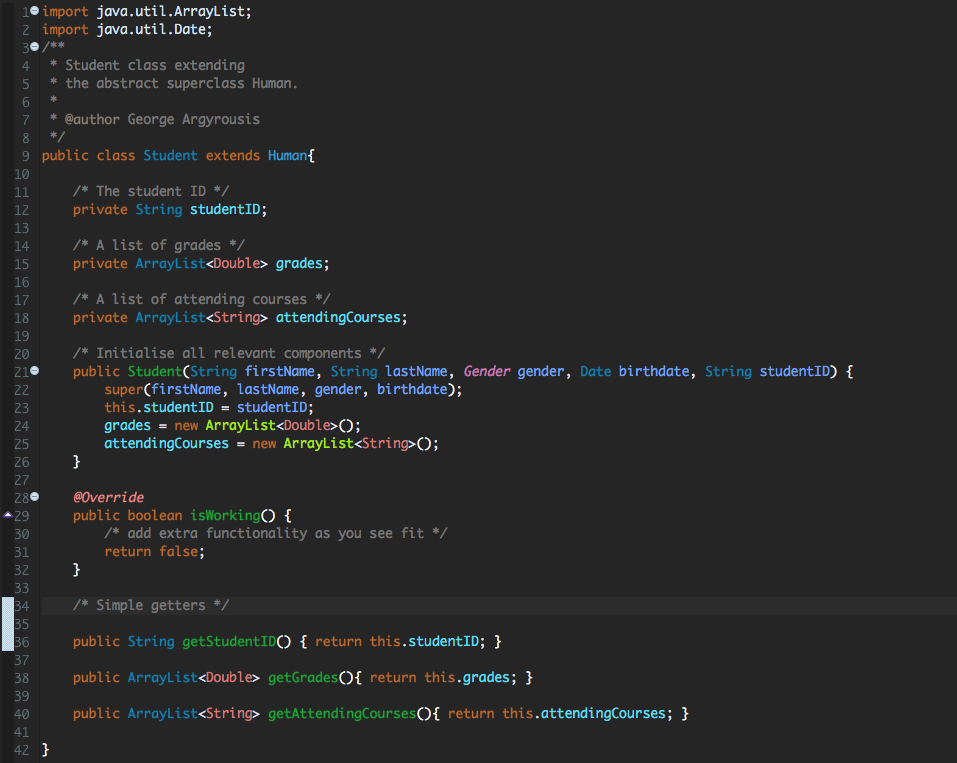
\includegraphics[scale=0.45]{images/Student_Step2.png}

            Last but not least, we initialize the object and print it's attributes in the command line.

            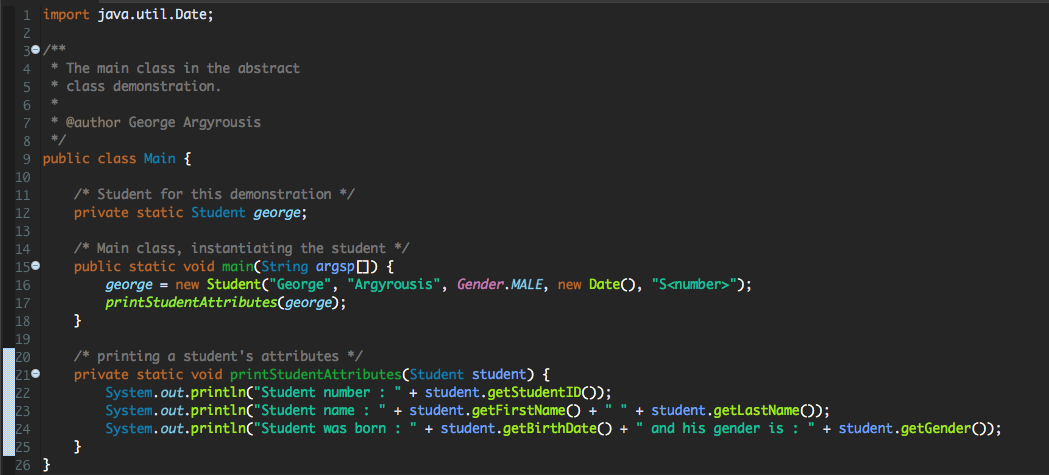
\includegraphics[scale=0.40]{images/Main_without_error.png}

            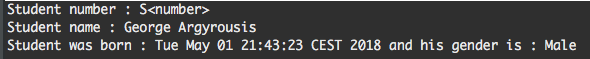
\includegraphics[scale=0.71]{images/output.png}

    \newpage

    \section{Interfaces}
    	\subsection{Definition}
    		\href{https://docs.oracle.com/javase/tutorial/java/concepts/interface.html}{Oracle Java Interface Tutorial}

    		In the most literal sense, an interface is a list of unimplemented methods that should all be related to each other.

    		When an object \textit{implements} an interface, it promises that it will provide behavior for the methods that the interface defines.

    		This allows for very useful behavior: Two potentially unrelated classes may implement a common interface, allowing them to be interpreted simply as two arbitrary objects that both have some common methods, thanks to the interface.

    		For example, suppose you are making a video game and need your player to interact with things that have items, like a chest, another player, an NPC, or perhaps some stones or trees. 

    		Without interfaces, we would have have each of these objects inherit from some superclass which defines how to take and give items to these objects. However, conceptually a player is not very related to a tree. 

    		To avoid some unintuitive inheritance structure, we can instead introduce an interface which defines methods such as \verb|takeItem(Item item)| and \verb|giveItem(Item item)|.

    		With our new \verb|Tradeable| interface, \textit{or whatever you want to name it, just something descriptive}, each of these objects can now promise that it will implement these methods so that they can be called on a player, a chest, an NPC, or a stone.


\end{document}
